\PassOptionsToPackage{unicode=true}{hyperref} % options for packages loaded elsewhere
\PassOptionsToPackage{hyphens}{url}
%
\documentclass[ignorenonframetext,]{beamer}
\usepackage{pgfpages}
\setbeamertemplate{caption}[numbered]
\setbeamertemplate{caption label separator}{: }
\setbeamercolor{caption name}{fg=normal text.fg}
\beamertemplatenavigationsymbolsempty
% Prevent slide breaks in the middle of a paragraph:
\widowpenalties 1 10000
\raggedbottom
\setbeamertemplate{part page}{
\centering
\begin{beamercolorbox}[sep=16pt,center]{part title}
  \usebeamerfont{part title}\insertpart\par
\end{beamercolorbox}
}
\setbeamertemplate{section page}{
\centering
\begin{beamercolorbox}[sep=12pt,center]{part title}
  \usebeamerfont{section title}\insertsection\par
\end{beamercolorbox}
}
\setbeamertemplate{subsection page}{
\centering
\begin{beamercolorbox}[sep=8pt,center]{part title}
  \usebeamerfont{subsection title}\insertsubsection\par
\end{beamercolorbox}
}
\AtBeginPart{
  \frame{\partpage}
}
\AtBeginSection{
  \ifbibliography
  \else
    \frame{\sectionpage}
  \fi
}
\AtBeginSubsection{
  \frame{\subsectionpage}
}
\usepackage{lmodern}
\usepackage{amssymb,amsmath}
\usepackage{ifxetex,ifluatex}
\usepackage{fixltx2e} % provides \textsubscript
\ifnum 0\ifxetex 1\fi\ifluatex 1\fi=0 % if pdftex
  \usepackage[T1]{fontenc}
  \usepackage[utf8]{inputenc}
  \usepackage{textcomp} % provides euro and other symbols
\else % if luatex or xelatex
  \usepackage{unicode-math}
  \defaultfontfeatures{Ligatures=TeX,Scale=MatchLowercase}
\fi
% use upquote if available, for straight quotes in verbatim environments
\IfFileExists{upquote.sty}{\usepackage{upquote}}{}
% use microtype if available
\IfFileExists{microtype.sty}{%
\usepackage[]{microtype}
\UseMicrotypeSet[protrusion]{basicmath} % disable protrusion for tt fonts
}{}
\IfFileExists{parskip.sty}{%
\usepackage{parskip}
}{% else
\setlength{\parindent}{0pt}
\setlength{\parskip}{6pt plus 2pt minus 1pt}
}
\usepackage{hyperref}
\hypersetup{
            pdftitle={305 Lecture 01 - Getting Started},
            pdfauthor={Brian Weatherson},
            pdfborder={0 0 0},
            breaklinks=true}
\urlstyle{same}  % don't use monospace font for urls
\newif\ifbibliography
\usepackage{graphicx,grffile}
\makeatletter
\def\maxwidth{\ifdim\Gin@nat@width>\linewidth\linewidth\else\Gin@nat@width\fi}
\def\maxheight{\ifdim\Gin@nat@height>\textheight\textheight\else\Gin@nat@height\fi}
\makeatother
% Scale images if necessary, so that they will not overflow the page
% margins by default, and it is still possible to overwrite the defaults
% using explicit options in \includegraphics[width, height, ...]{}
\setkeys{Gin}{width=\maxwidth,height=\maxheight,keepaspectratio}
\setlength{\emergencystretch}{3em}  % prevent overfull lines
\providecommand{\tightlist}{%
  \setlength{\itemsep}{0pt}\setlength{\parskip}{0pt}}
\setcounter{secnumdepth}{0}

% set default figure placement to htbp
\makeatletter
\def\fps@figure{htbp}
\makeatother

\let\Tiny=\tiny

 \setbeamertemplate{navigation symbols}{} 

% \usetheme{Madrid}
 \usetheme[numbering=none, progressbar=foot]{metropolis}
 \usecolortheme{wolverine}
 \usepackage{color}
 \usepackage{MnSymbol}
% \usepackage{movie15}

\usepackage{amssymb}% http://ctan.org/pkg/amssymb
\usepackage{pifont}% http://ctan.org/pkg/pifont
\newcommand{\cmark}{\ding{51}}%
\newcommand{\xmark}{\ding{55}}%

\DeclareSymbolFont{symbolsC}{U}{txsyc}{m}{n}
\DeclareMathSymbol{\boxright}{\mathrel}{symbolsC}{128}
\DeclareMathAlphabet{\mathpzc}{OT1}{pzc}{m}{it}


% \usepackage{tikz-qtree}
% \usepackage{markdown}
% \usepackage{prooftrees}
% \forestset{not line numbering, close with = x}
% Allow for easy commas inside trees
\renewcommand{\,}{\text{, }}


\usepackage{tabulary}

\usepackage{open-logic-config}

\setlength{\parskip}{1ex plus 0.5ex minus 0.2ex}

\AtBeginSection[]
{
\begin{frame}
	\Huge{\color{darkblue} \insertsection}
\end{frame}
}

\renewenvironment*{quote}	
	{\list{}{\rightmargin   \leftmargin} \item } 	
	{\endlist }

\definecolor{darkgreen}{rgb}{0,0.7,0}
\definecolor{darkblue}{rgb}{0,0,0.8}

\newcommand{\starttab}{\begin{center}
\vspace{6pt}
\begin{tabular}}

\newcommand{\stoptab}{\end{tabular}
\vspace{6pt}
\end{center}
\noindent}


\newcommand{\sif}{\rightarrow}
\newcommand{\siff}{\leftrightarrow}
\newcommand{\EF}{\end{frame}}


\newcommand{\TreeStart}[1]{
%\end{frame}
\begin{frame}
\begin{center}
\begin{tikzpicture}[scale=#1]
\tikzset{every tree node/.style={align=center,anchor=north}}
%\Tree
}

\newcommand{\TreeEnd}{
\end{tikzpicture}
%\end{center}
}

\newcommand{\DisplayArg}[2]{
\begin{enumerate}
{#1}
\end{enumerate}
\vspace{-6pt}
\hrulefill

%\hspace{14pt} #2
%{\addtolength{\leftskip}{14pt} #2}
\begin{quote}
{\normalfont #2}
\end{quote}
}

\newenvironment{ProofTree}[1][1]{
\begin{center}
\begin{tikzpicture}[scale=#1]
\tikzset{every tree node/.style={align=center,anchor=south}}
}
{
\end{tikzpicture}
\end{center}
}

\newcommand{\TreeFrame}[2]{
\begin{columns}[c]
\column{0.5\textwidth}
\begin{center}
\begin{prooftree}{}
#1
\end{prooftree}
\end{center}
\column{0.45\textwidth}
%\begin{markdown}
#2
%\end{markdown}
\end{columns}
}

\newcommand{\ScaledTreeFrame}[3]{
\begin{columns}[c]
\column{0.5\textwidth}
\begin{center}
\scalebox{#1}{
\begin{prooftree}{}
#2
\end{prooftree}
}
\end{center}
\column{0.45\textwidth}
%\begin{markdown}
#3
%\end{markdown}
\end{columns}
}

\usepackage[bb=boondox]{mathalfa}
\DeclareMathAlphabet{\mathbx}{U}{BOONDOX-ds}{m}{n}
\SetMathAlphabet{\mathbx}{bold}{U}{BOONDOX-ds}{b}{n}
\DeclareMathAlphabet{\mathbbx} {U}{BOONDOX-ds}{b}{n}

\RequirePackage{bussproofs}
\RequirePackage[tableaux]{prooftrees}

\newenvironment{oltableau}{\center\tableau{}} %wff format={anchor = base west}}}
       {\endtableau\endcenter}
       
\newcommand{\formula}[1]{$#1$}

\usepackage{tabulary}
\usepackage{booktabs}

\def\begincols{\begin{columns}}
\def\begincol{\begin{column}}
\def\endcol{\end{column}}
\def\endcols{\end{columns}}

\usepackage[italic]{mathastext}
\usepackage{nicefrac}

\definecolor{mygreen}{RGB}{0, 100, 0}
\definecolor{mypink2}{RGB}{219, 48, 122}
\definecolor{dodgerblue}{RGB}{30,144,255}

\def\True{\textcolor{dodgerblue}{\text{T}}}
\def\False{\textcolor{red}{\text{F}}}

\title{305 Lecture 01 - Getting Started}
\author{Brian Weatherson}
\date{July 1, 2020}

\begin{document}
\frame{\titlepage}

\begin{frame}{Aim of Course}
\protect\hypertarget{aim-of-course}{}

Introductory survey of some formal methods that are of broad
philosophical use.

\end{frame}

\begin{frame}{Three Sections}
\protect\hypertarget{three-sections}{}

\begin{enumerate}
\tightlist
\item
  Propositional Logic
\item
  Probability and Statistical Reasoning
\item
  Modal Logic and Conditionals
\end{enumerate}

\end{frame}

\begin{frame}{Propositional Logic}
\protect\hypertarget{propositional-logic}{}

\begin{itemize}[<+->]
\tightlist
\item
  This is the logic of sentences that can be true or false, and that can
  combine to form longer sentences.
\item
  It is taken for granted in almost any field (outside philosophy) where
  formal tools are used.
\item
  In philosophy we might sometimes want to drop the assumption that
  everything is either true or false (and not both), but for this course
  we'll take it for granted.
\end{itemize}

\end{frame}

\begin{frame}{Probability and Statistical Reasoning}
\protect\hypertarget{probability-and-statistical-reasoning}{}

\begin{itemize}[<+->]
\tightlist
\item
  Sometimes we can't infer that a conclusion is definitely true, but we
  can infer that it is probably true.
\item
  We will look at some tools for regimenting how and when we make such
  inference.
\end{itemize}

\end{frame}

\begin{frame}{Modal Logic}
\protect\hypertarget{modal-logic}{}

This is the logic of `must' and `might'. It has as many applications as
there are interpretations of `must' and `might'. The primary
interpretations we'll look at are:

\begin{itemize}
\tightlist
\item
  Metaphysical
\item
  Epistemological\\
\item
  Moral
\end{itemize}

\end{frame}

\begin{frame}{Textbooks}
\protect\hypertarget{textbooks}{}

There are three - all of them available through Canvas.

\begin{enumerate}
\tightlist
\item
  \emph{The Carnap Book} by Graham Leach-Krouse
\item
  \emph{Odds and Ends} by Jonathan Weisberg
\item
  \emph{Boxes and Diamonds, Ann Arbor remix}
\end{enumerate}

The three books are for the three parts of the course.

\end{frame}

\begin{frame}{The Carnap Book}
\protect\hypertarget{the-carnap-book}{}

\begin{figure}
\centering
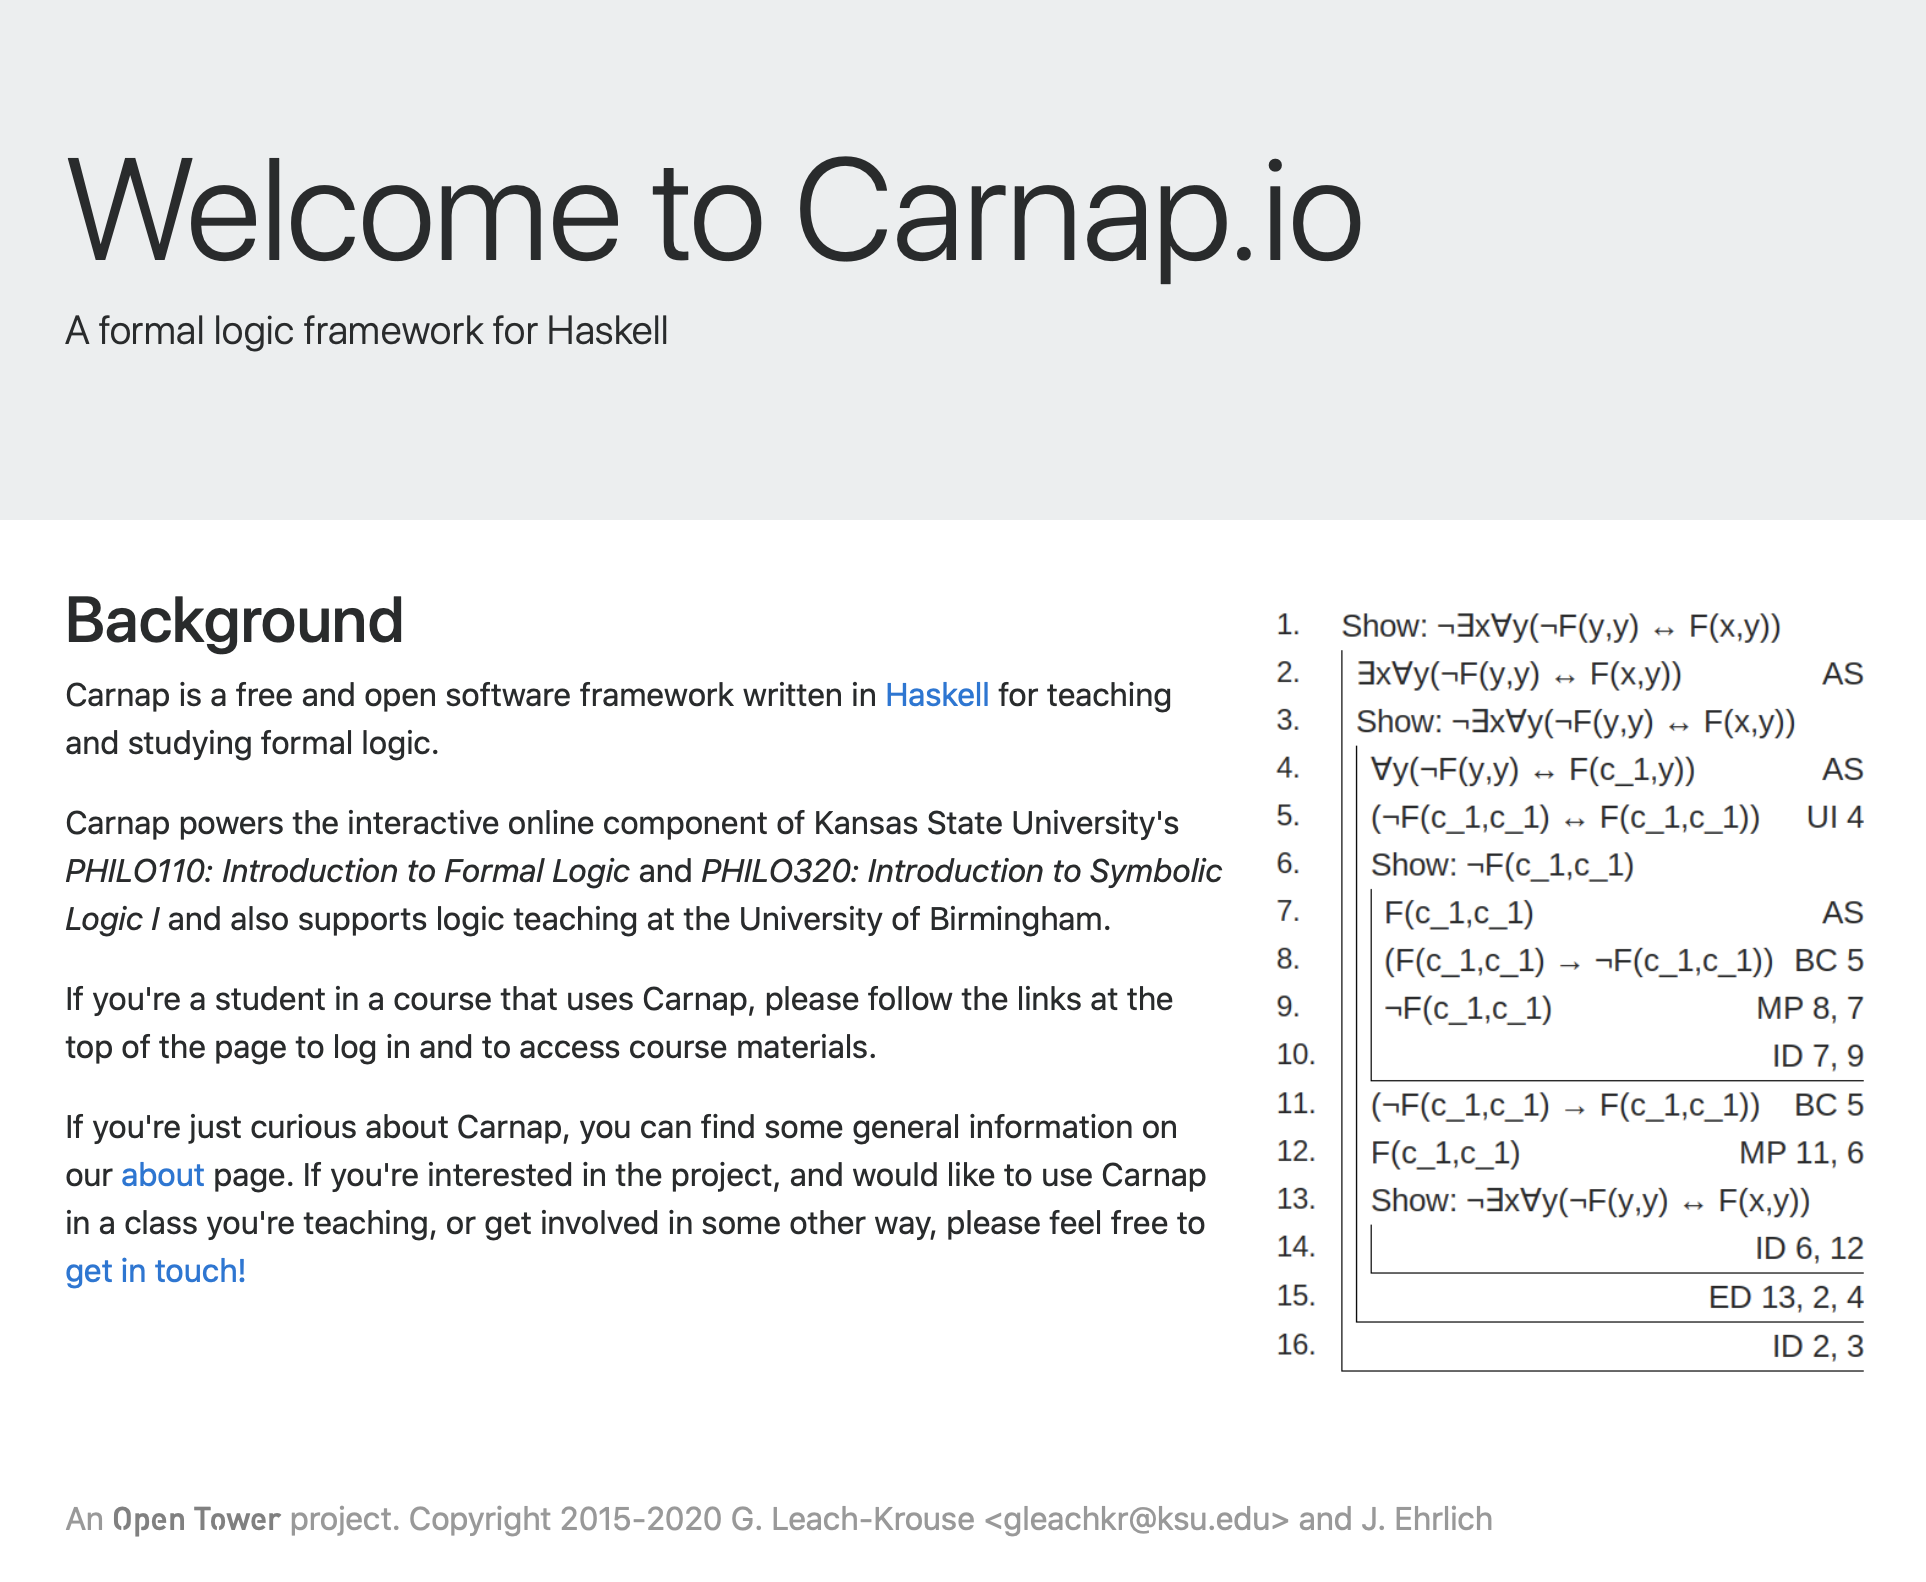
\includegraphics[width=\textwidth,height=0.8\textheight]{images/0_1_a_Carnap.png}
\caption{\url{https://carnap.io}}
\end{figure}

\end{frame}

\begin{frame}{Registering with Carnap}
\protect\hypertarget{registering-with-carnap}{}

\begin{figure}
\centering

\includegraphics[width=\textwidth,height=0.8\textheight]{images/0_1_a_Carnap_Need_Register.png}
\caption{One more registration step}
\end{figure}

\end{frame}

\begin{frame}

\begin{figure}
\centering
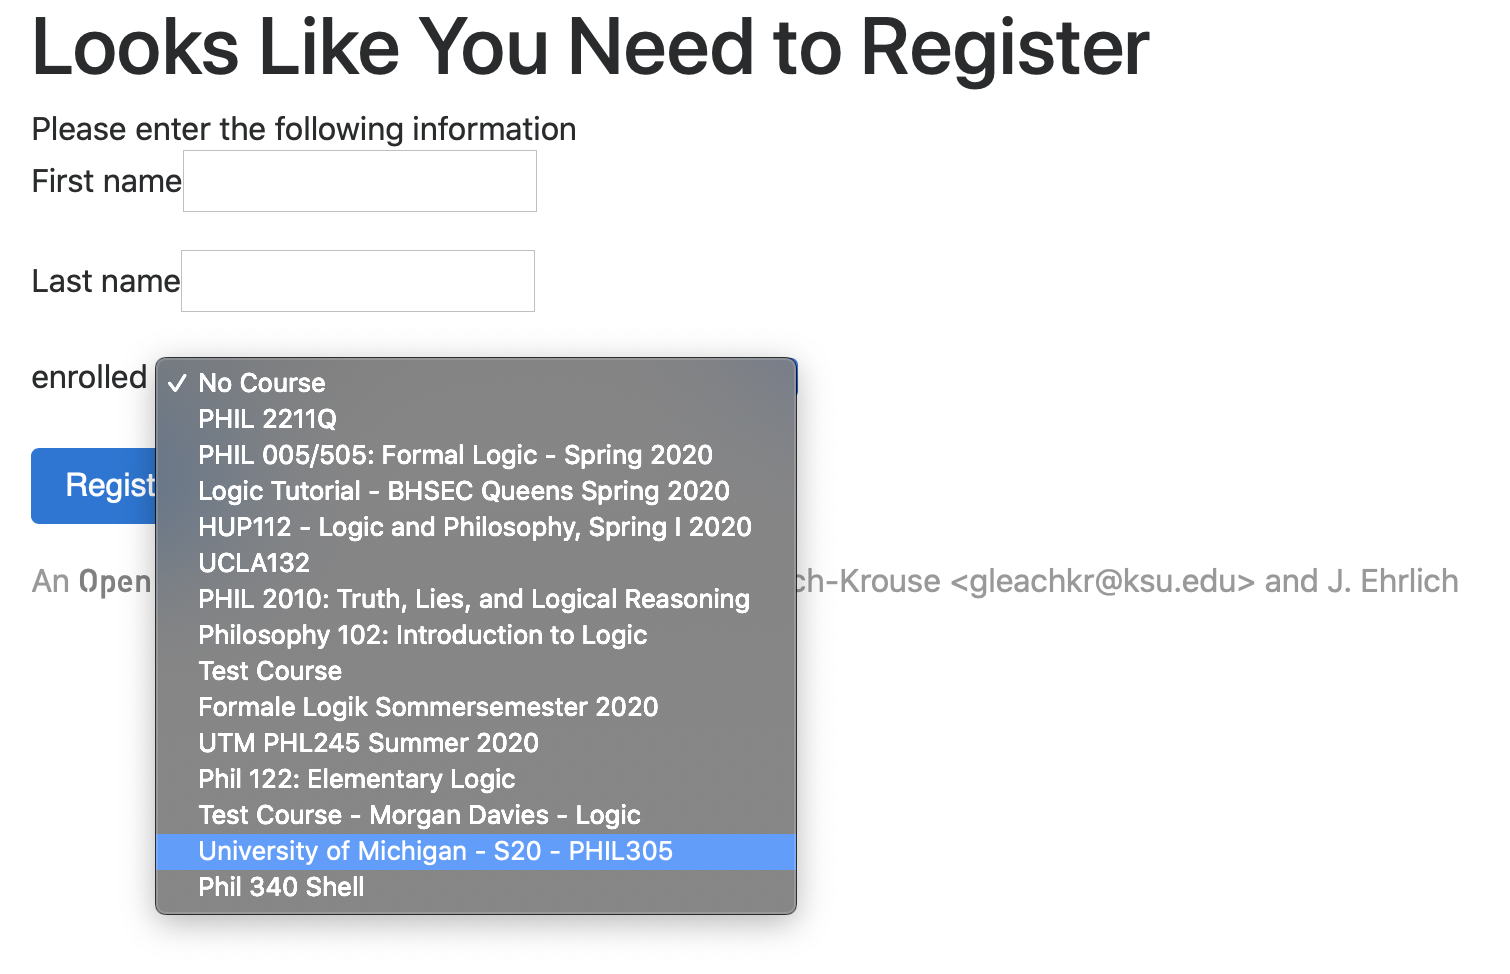
\includegraphics[width=\textwidth,height=0.8\textheight]{images/0_1_a_Registration.png}
\caption{Register in the right course}
\end{figure}

\end{frame}

\begin{frame}{Odds and Ends}
\protect\hypertarget{odds-and-ends}{}

\begin{figure}
\centering
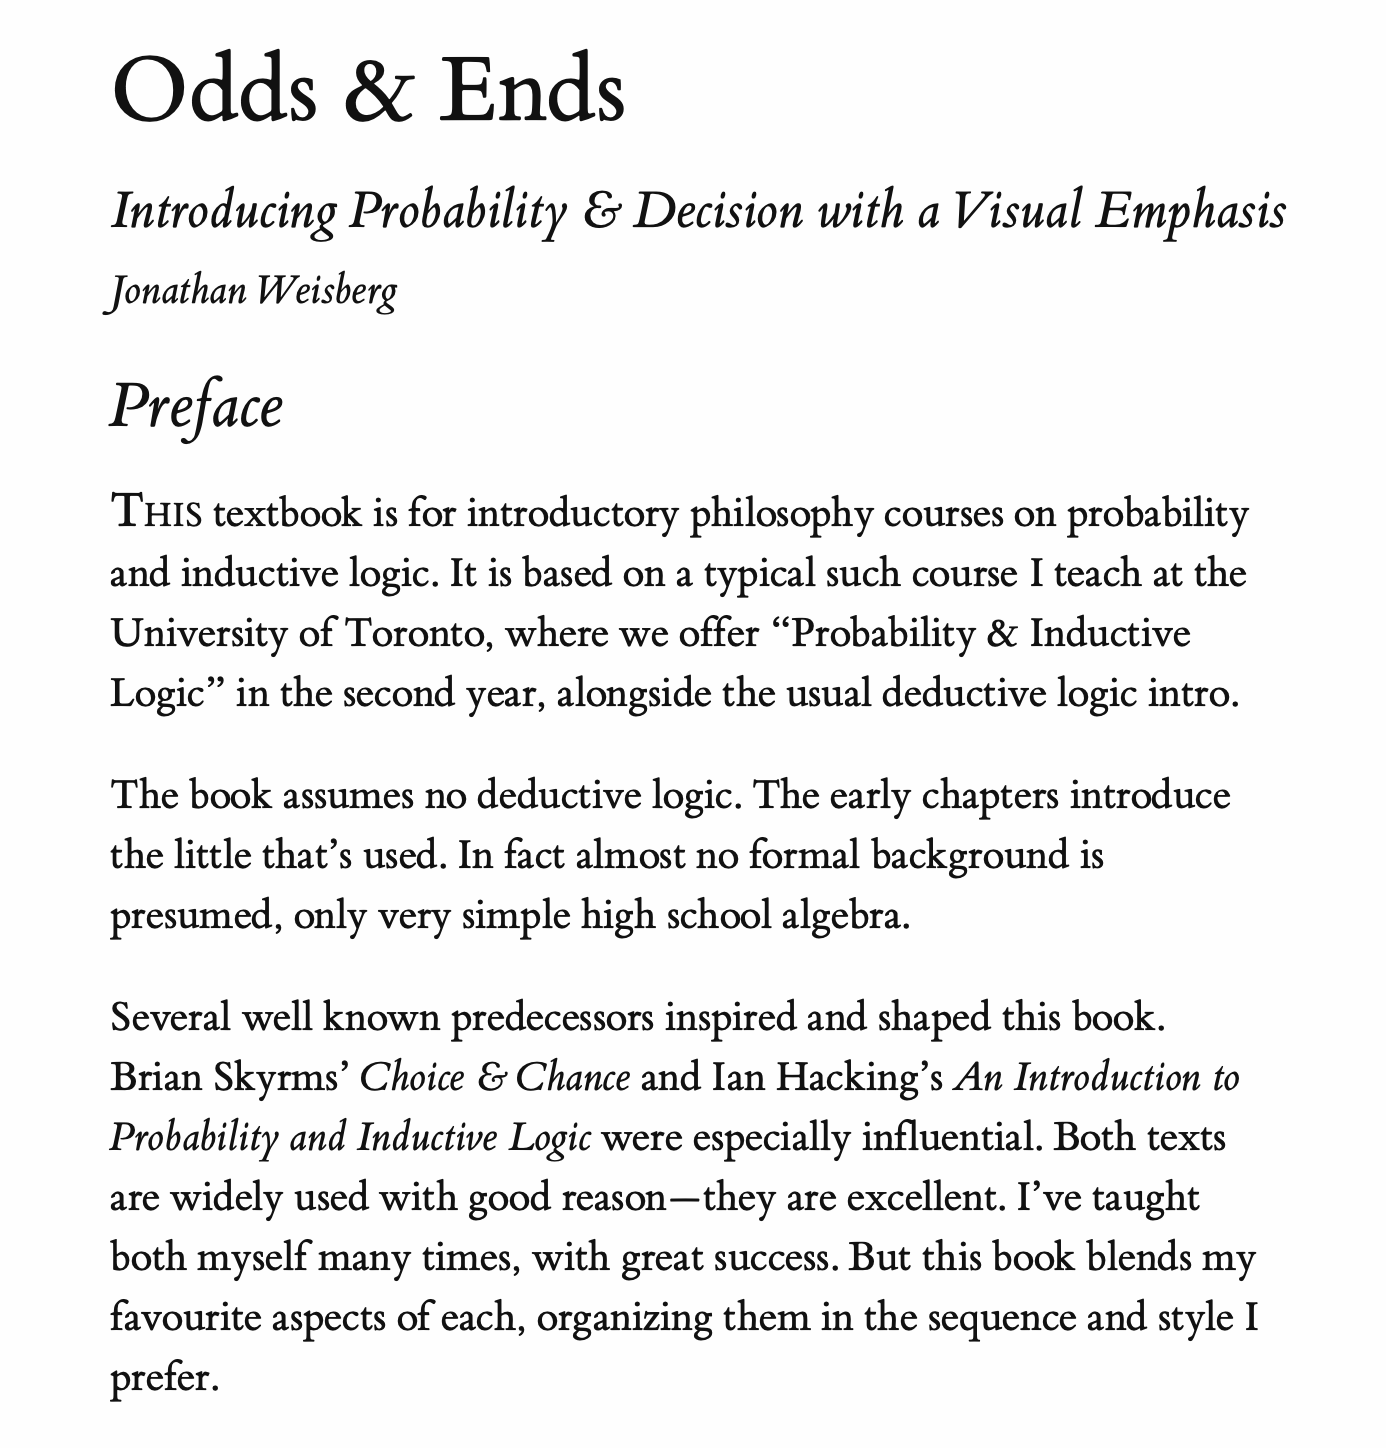
\includegraphics[width=\textwidth,height=0.8\textheight]{images/0_1_a_Odds_and_Ends.png}
\caption{\url{https://jonathanweisberg.org/vip/}}
\end{figure}

\end{frame}

\begin{frame}{Boxes and Diamonds}
\protect\hypertarget{boxes-and-diamonds}{}

\begin{figure}
\centering
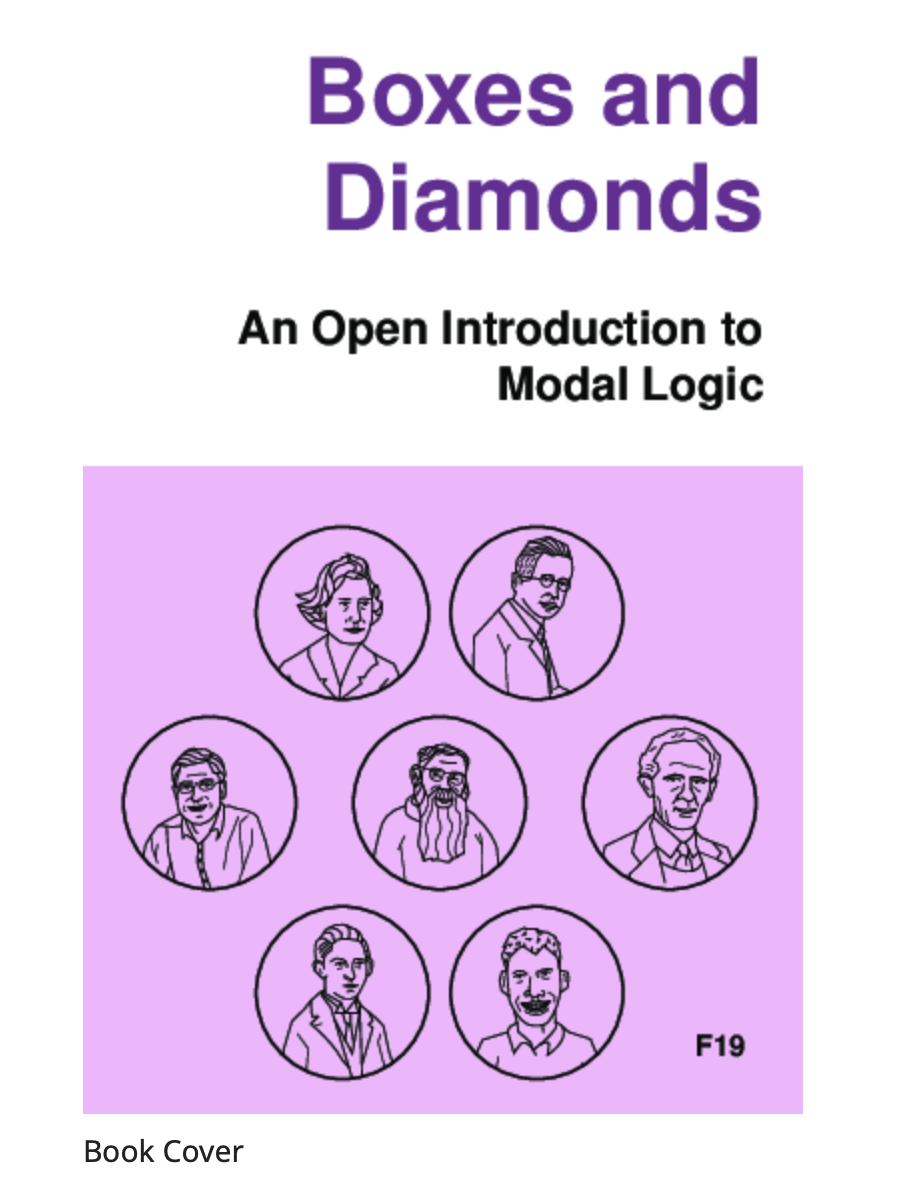
\includegraphics[width=\textwidth,height=0.8\textheight]{images/0_1_a_Boxes_and_Diamonds.png}
\caption{\url{https://bd.openlogicproject.org}}
\end{figure}

\end{frame}

\begin{frame}

\begin{figure}
\centering
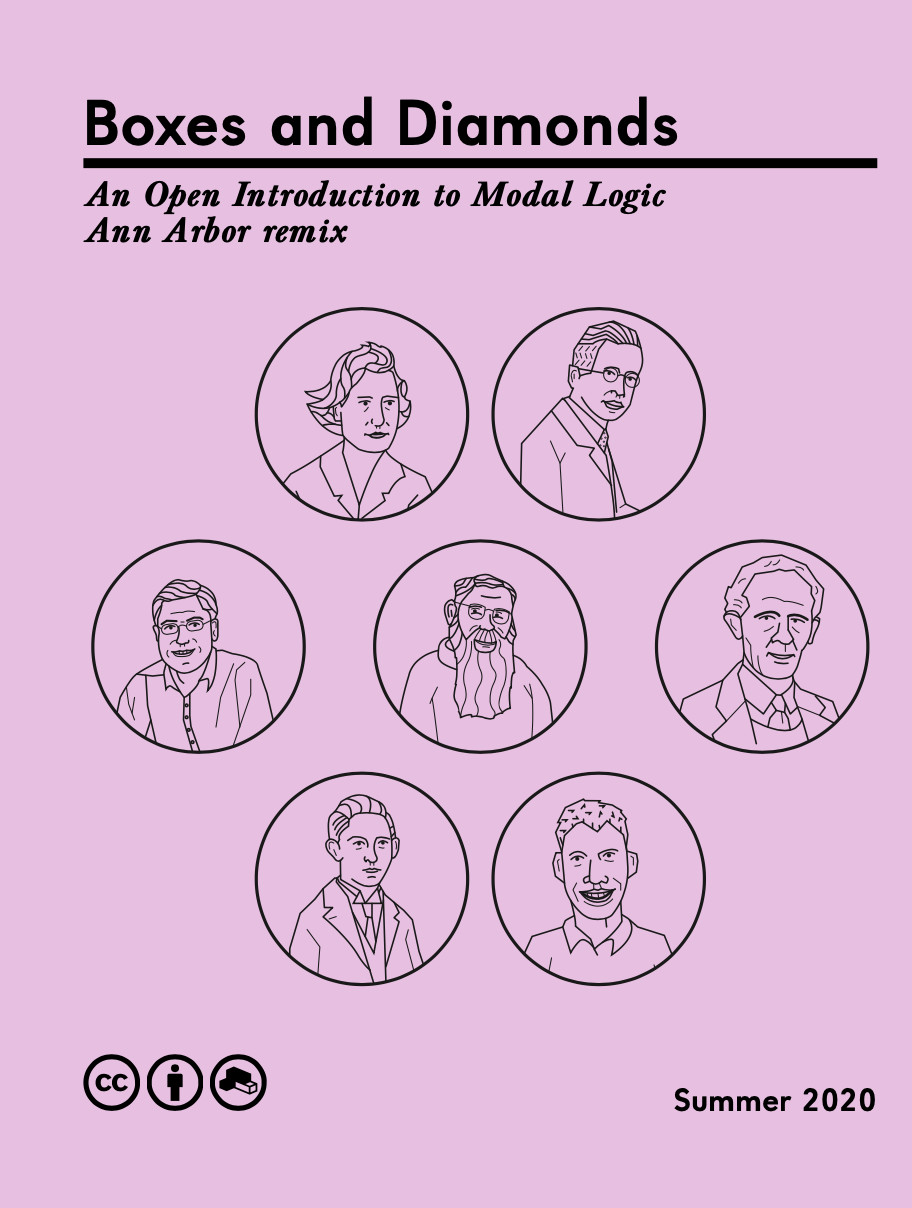
\includegraphics[width=\textwidth,height=0.8\textheight]{images/0_1_a_Boxes_and_Diamonds_AA.png}
\caption{Boxes and Diamonds - Ann Arbor}
\end{figure}

\end{frame}

\end{document}
